%!TEX root = main.tex

\chapter{Implementation}
In this chapter we describe how we implemented the project.
In Section \ref{sec:overview} we explain why we did what we did.
In Section \ref{sec:integration} we explain how we integrated BWAPI with LIDA.
Section \ref{sec:detectors} explains the feature detectors we made.
In Section \ref{sec:attention} we explain how we manage attention in our agent.
In Section \ref{sec:actionexecution} we explain how action are executed.

\section{Overview}
\label{sec:overview}
We chose to use the LIDA framework because it is built on a strong theoretical foundation of core cognitive principals. Even though the framework is currently, at the time of this writing, only in a beta version it is well-documented and has an active community working on improving it. Because LIDA is written in Java we had to use JNI-BWAPI since it provides Java bindings for BWAPI.

We made the decision to allow our agent access to perfect information about the environment in StarCraft, this means that it can see the whole map and all the units on the map without having to scout first. We did this because it simplified our implementation and made it easier to begin with to create an agent that functioned decently. With the same reasoning in mind, we decided that we would go for a simple strategy in our games, and limit our self to only use one race. So we decided to use the Protoss race, and our strategy involved building gateways, that are the the basic unit production building for Protoss, and then producing an army consisting of Zealots, a basic close-range melee unit.

\section{Integration}
\label{sec:integration}
BWAPI itself provides only a basic C++ API, so JNIBWAPI provides, as explained in Chapter \ref{sec:starcrafttheory}, a custom Java API using the Java Native Interface, JNI.\cite{jni} Because we can't load an entire Java VM into the StarCraft process, we use shared memory to connect the StarCraft process with the process of our agent. Because the processes manipulates the same shared memory area both processes needs to be ran with Administrator privileges in Windows.

We also updated JNIBWAPI to adapt to some minor recent changes in BWAPI, and added in some missing functionality that we needed for controlling the game, like starting, pausing and restarting the on-going game.

In order to use the LIDA framework we had to integrate LIDA with JNIBWAPI. To accomplish this we implement the domain specific modules of the LIDA framework to make calls to JNIBWAPI.

\begin{figure}[h!tb]
\centering
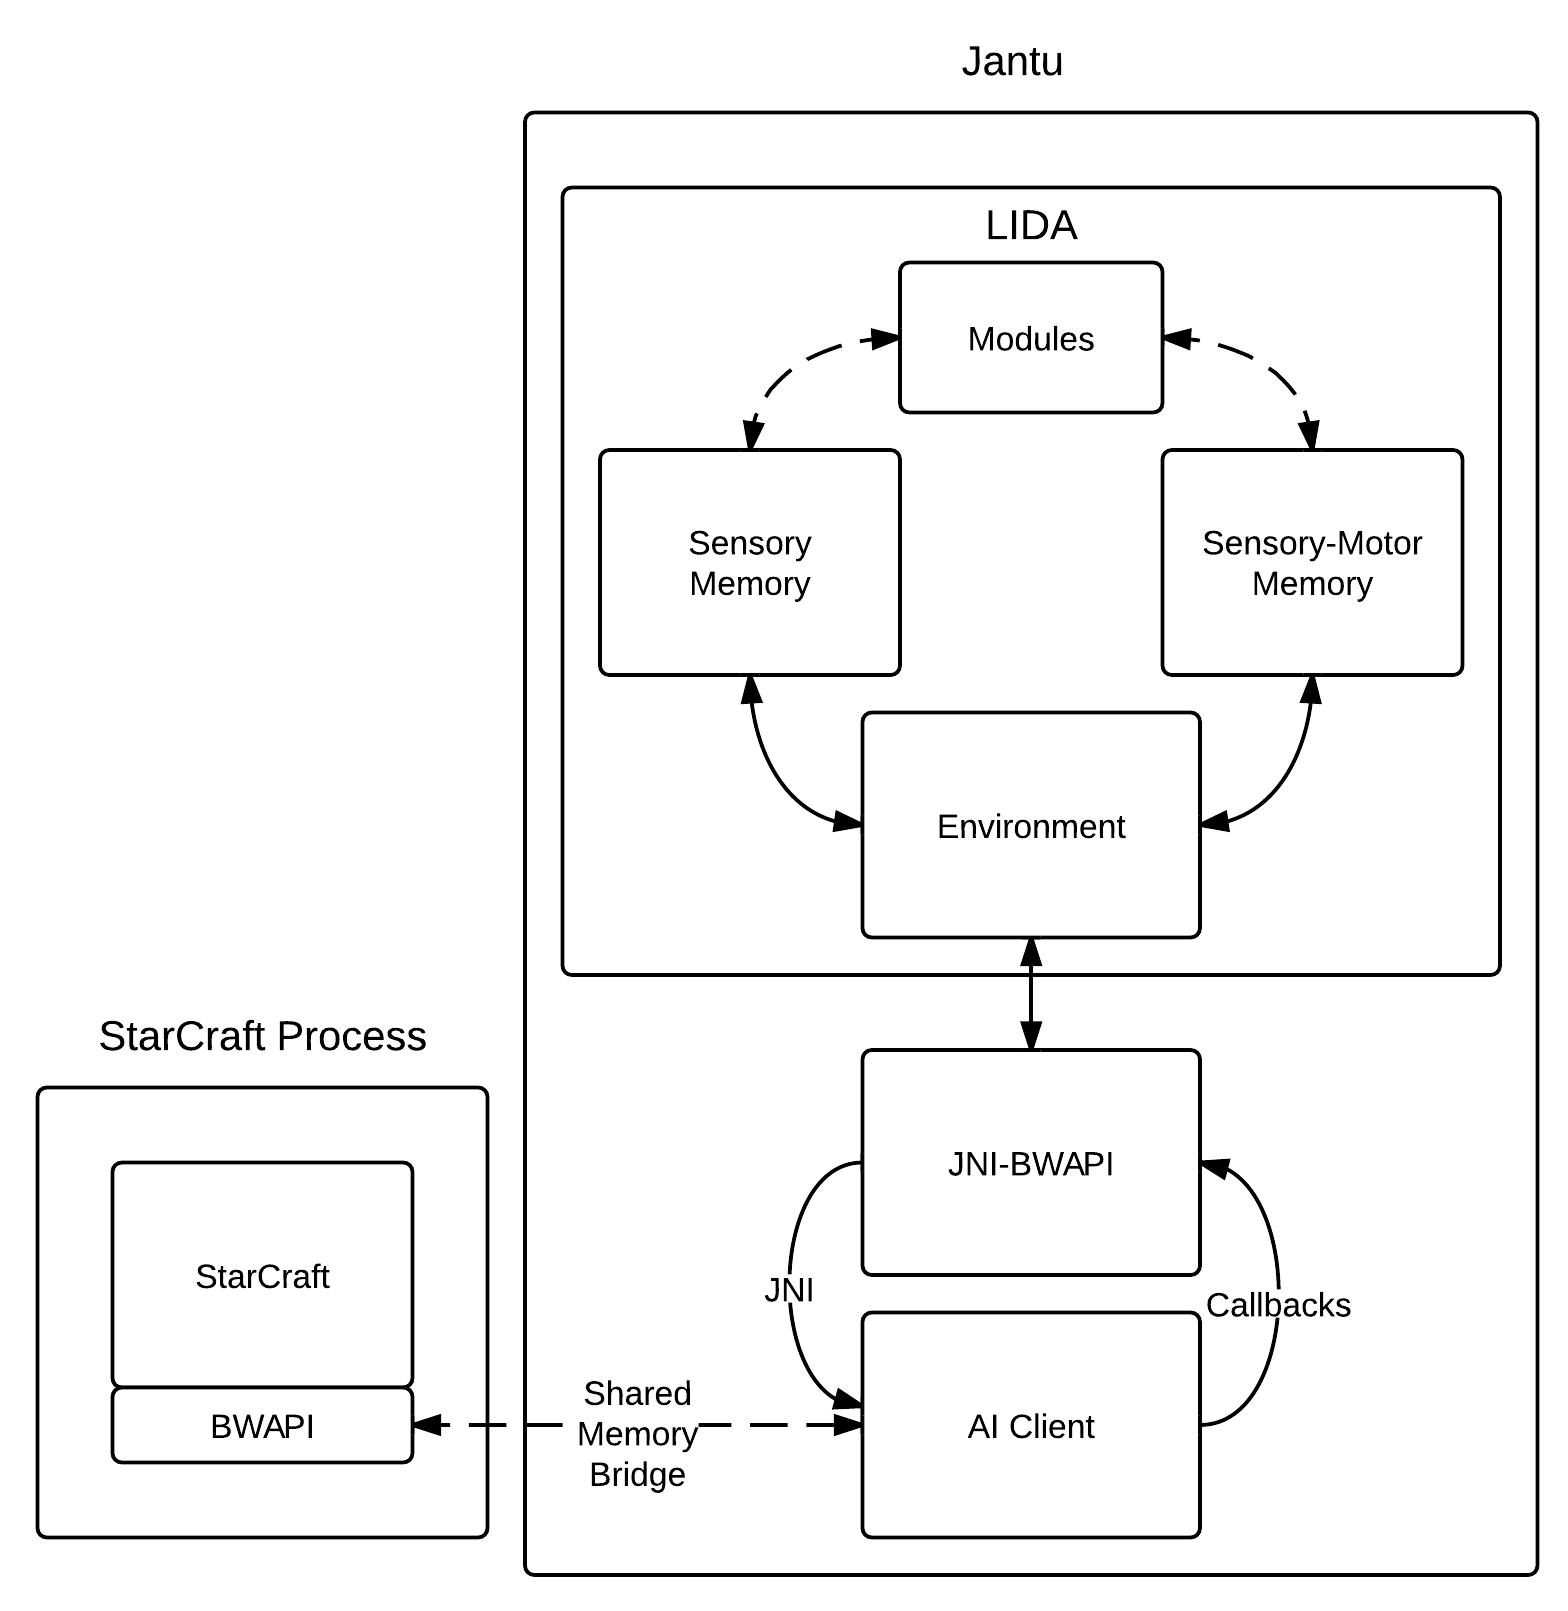
\includegraphics[scale=1.0]{graphics/jantu.png}
\caption{A general architecture overview of Jantu}
\label{fig:jantu}
\end{figure}

Figure \ref{fig:jantu} shows a general overview of the Jantu bot's architecture, which consists of 3 main parts. In the StarCraft process the game itself runs together with BWAPI injected into the game client. Because our code needs to be run in the Java virtual machine, our code is run in a separate process that communicates with the Starcraft process using a shared memory bridge. This enables JNI-BWAPI to make calls to BWAPI and retrieve information back across the bridge.

In the Jantu process JNI-BWAPI is running together with the LIDA framework. In order to integrate the LIDA framework with JNI-BWAPI we setup the framework first with the configurations we needed to get it up and running. This involves describing and structuring the modules you need in different XML configuration files. Also in these files we configure what kind of information that will be possible to use and transmit internally in the LIDA framework.

JNI-BWAPI consists of different models and types that represent Starcraft information like units and buildings together with a lot of native functions that can be called to communicate with BWAPI. We integrated this with LIDA by using a custom implementation of the Environment class in LIDA. This class becomes the interface between the domain specific modules of LIDA, the sensory memory and sensory-action memory, and JNI-BWAPI.


\subsubsection{Environment module}
The Environment module is the interface between JNI-BWAPI and LIDA. It is responsible for abstracting away the JNI-BWAPI, and making sure that the game runs when it should. It allows LIDA to reset the state of the environment, by restarting the game.

\paragraph{Timing} When working with a cognitive architecture it is important to be able to look at the internal structures of the model during runtime, like the current situation model and what node structures have what activations. This is useful for debugging and performance tweaking.

To achieve this we have to be able to pause and resume the game at any time, so to get the run/pause and timing functionality of LIDA inside StarCraft, we have a semaphore\footnote{A semaphore is a special data structure that is used for synchronization of threads. It has a number of {\em permits}, which a thread can request. A thread will pause while waiting for an available permit. Another thread can then release permits in the semaphore to let the waiting threads continue.} that is released by a LIDA codelet each tick, and then the callback from StarCraft/BWAPI that we get each frame waits for this to be released. This allows us to easily set the amount of StarCraft frames that are processed for each LIDA cycle, by increasing the amount of permits available in the semaphore. In our implementation we let one cognitive cycle equate to one in-game frame.

\paragraph{GUI panel} We also provide a custom GUI panel to represent the environment, see Figure \ref{fig:environment-gui}. Different regions from the Brood War Terrain Analyzer are separated by gray lines. Enemy entities are displayed as red dots, entities owned by our agent are blue dots. Neutral entities (vespene geysers and mineral fields) are green. Choke points are marked by yellow circles.

\begin{figure}[h!tb]
\centering
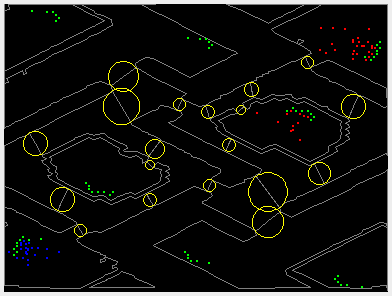
\includegraphics{graphics/environment-gui.png}
\caption{Our custom representation of the state of the environment.}
\label{fig:environment-gui}
\end{figure}

\section{Detectors}
\label{sec:detectors}
Feature detectors are how LIDA perceives it's environment and identifies important aspects of the current game state. They are tasks that are run repeatedly, at specific intervals and parses the game state at that time in order to identify a given feature that can later be used in different modules in LIDA, to recognize thoughts and concepts. Each detector usually only identifies one specific feature, but it is possible for one detector to identify several features if they are of the same type.

Feature detectors can be created that detect almost every aspect of the game, and they can be everything from simply detecting the existence of specific units or game elements to more complex detectors that detect army compositions or enemy tactics and strategies. The more of them you implement the more advanced concepts you can identify and that opens up more advanced strategies you can perform yourself.

\subsection{Implemented feature detectors}
Following are brief descriptions of the detectors we have implemented.

\subsubsection{IdleWorkerFeatureDetector}
Identifies worker units that don't have a job. A worker could be gathering resources, constructing buildings or scouting, and for efficiency it should be doing something at all times.

\subsubsection{ResourceFeatureDetector}
Identifies what type of units and buildings that we currently have enough resources available to create. This can be buildings we can construct, units we can morph or upgrades that we can research.

\subsubsection{SupplyBlockFeatureDetector}
Identifies when we are getting close to being supply blocked, that means that we can't build any more units until another supply-granting building/unit is created.

\subsubsection{UnsaturatedResourcesFeatureDetector}
Identifies whether or not our available resource nodes have are saturated with enough workers that are gathering them. This can be used to decide if we need to build more workers or not.

\subsubsection{BuildOrderFeatureDetector}
Identifies what type of building we need to construct for our next step in the planned build order. For our simple implementation it detects if we have more resource generation then unit production buildings, so we need to expand our capacity by adding new ones.

\subsubsection{IdleProductionFeatureDetector}
Identifies when a production building is currently not training any units. In StarCraft being effective with the resources you have available is important, therefore not queuing units on a production building is important, but instead only building new units when production buildings are idle.

\subsubsection{StructureFeatureDetector}
Identifies the buildings we have. This is important to know because we might not want to build another of the same building, and for unit production it is important to know what kind of production buildings we have available.

\subsubsection{TimingAttackFeatureDetector}
Identifies when it is time to attack the enemy. In our current implementation is a very simple detector that just waits until we have collected a substantial army of units and then activates to ``detect'' that it is now time to attack.

\section{Attention Module}
\label{sec:attention}
One of the main features of a cognitive system, and even of the human brain, is the ability to focus consciousness or give attention to a subsection of world as it perceives it. This is what the {\em attention module} is responsible for. It achieves this by running attention codelets that look for specific workspace content from the current situational model and them creates coalitions from this that are added to the global workspace, where they will compete with other coalitions for conscious focus.

The activation for a coalition is based both on the activation for the PAM nodes that it contains and the activation for the codelet itself that created it.

\subsection{Implemented attention codelets}
\subsubsection{Idle worker codelet}
A simple codelet that makes a coalition with idle worker node. This codelet has a high activation in order to make sure has a big change of winning the competition for consciousness since it is important for workers to be doing something at all times.

\subsubsection{Build worker codelet}
This codelet looks for three different situations that decides if a worker should be created. These are if we can afford to create the worker, if our resources are not saturated already and the base building is not currently training any units.

\subsubsection{Build supply codelet}
This is another simple but important codelet that has a high activation value. It looks for the situation where we are supply blocked, or getting close to being supply blocked, and we can afford to build a supply structure. It has a high activation level because getting supply blocked means you can't create any more units until another supply structure is finished building, that will be a lot of valuable time lost where no units is trained.

\subsubsection{Build Order Codelet}
This is one of the more complex codelets, it looks for all the buildings that we can currently afford as well as all the buildings that we need to create according to the build order nodes. Combining these in a coalition allows the action selector later to decide what building should be created next.

\subsubsection{Train Units Codelet}
This codelet is similar to the Build Order Codelet, except it looks for the units we can afford to train in addition to what unit production buildings we currently have available to use.

\subsubsection{Strategy Codelet}
This codelet looks for any node that is a child from the strategy node. These are defensive or offensive strategies during a game. In our implementation we only have a simple strategy that is to attack with every army unit we have at the same time, when we feel we have a sufficient army size.

\section{Action Execution}
\label{sec:actionexecution}
After LIDA has selected a focus of consciousness and an appropriate action has been selected from the behavior net, the selected action must be executed. This gets executed by having the sensory-motor memory make function calls to the environment class, which functions as a bridge between LIDA and JNI-BWAPI.

How the action is implemented in the sensory-memory is up to the developer, as long as it performs its given function. It can be really simple implementation or you could do something more complex, LIDA is there to decide what parts or game state to focus on, and to make the decision on what action to perform, not how that action is executed.

\subsection{Implemented actions}
\subsubsection{Mine minerals}
This actions takes a worker that is not currently performing a task and orders it to start mining minerals from an unsaturated mineral deposit.

\subsubsection{Build worker}
This action starts training a worker unit at the main building in the home base, the Nexus for Protoss.

\subsubsection{Build supply}
This action constructs a building or unit that grants increased supply. This can be a building or a unit depending on the race. For Protoss it creates a structure called a pylon that grants more available maximum supply.

\subsubsection{Build gateway}
This action works in much the same way as {\em Build supply} except that it creates a production building called gateway. This building is used to warp in (train) army units.

\subsubsection{Train zealot}
This action sets a zealot for training at an available gateway that is currently not training any other units. It is important that it doesn't queue it at a gateway that is already training another unit since it locks up resources and is inefficient.

\subsubsection{Attack}
This action executes an attack on enemy units. It can be a very simple action like in our implementation where it just used every available army unit and attacks the enemy, or it could be more complex like using groups of units for different attacks. Also worth noting that if you are not using perfect information then you can only attack units that you have seen by scouting, you are being invaded by or otherwise manage to see.
